\documentclass[a4paper,12pt]{book}

\usepackage{url}
\usepackage[brazil]{babel}
\usepackage[pdftex]{graphicx}
\usepackage[pdftex]{hyperref}

\title{Laborat\'orio de Programa\c c\~ao II - Fase zero do projeto}
\author{
		Douglas Bettioli Barreto (NUSP 6920223)
		\and Giancarlo Rigo (NUSP 6910034)
		\and Rafael Reggiani Manzo (NUSP 6797150)
	   }

\begin{document}

\maketitle

\section{Proposta de Jogo}
\subsection{Como \'e}
\label{sec: comoeojogo}

O grupo se prop\~oe a implementar um jogo de xadrez com op\c c\~ao de jogo para
duas pessoas ou uma pessoa contra uma engine de xadrez (talvez escolhamos uma
opensource ou implementaremos nossa pr\'opria de forma mais simples).

A realidade aumentada entra onde o jogador deve movimentar, ao inv\'es de pe\c
cas, tags que ser\~ao filmadas pela webcam, reconhecidas pelo software,
interpretadas e desenhadas.

\subsection{Como se joga}
\label{sec: comosejoga}

O jogo deve seguir a maior parte das regras do xadrez original que podem ser
encontradas em \url{http://en.wikipedia.org/wiki/Rules_of_chess}. Algumas
regras como ``Pe\c ca tocada \'e pe\c ca jogada'' n\~ao pretendemos
implementar, pois, al\'em de serem consistirem em eventos dif\'iceis de se
detectar, tornam o jogo mais ``chato'' de um certo ponto de vista.

\subsection{Cen\'ario}
\label{sec: cenario}

N\~ao teremos um cen\'ario propriamente dito, mas o equivalente a isto ser\'a um
tabuleiro especial sempre composto de 64 tags, que podem ou n\~ao se repetir.

Este tabuleiro ser\'a interpretado pelo software que desenhar\'a o tabuleiro e
as pe\c cas que estiverem nele de acordo com as tags que forem identificadas.

Tanto o tabuleiro visto a olho n\'u, como o tabuleiro visto atrav\'es do
software est\~ao ilustrados nos esbo\c cos das telas do jogo (\ref{sec: telas}).

\section{Esbo\c co das telas do jogo}
\label{sec: telas}

\subsection{Menu}
\label{subsec: menu}

\begin{figure}[h]
\centering
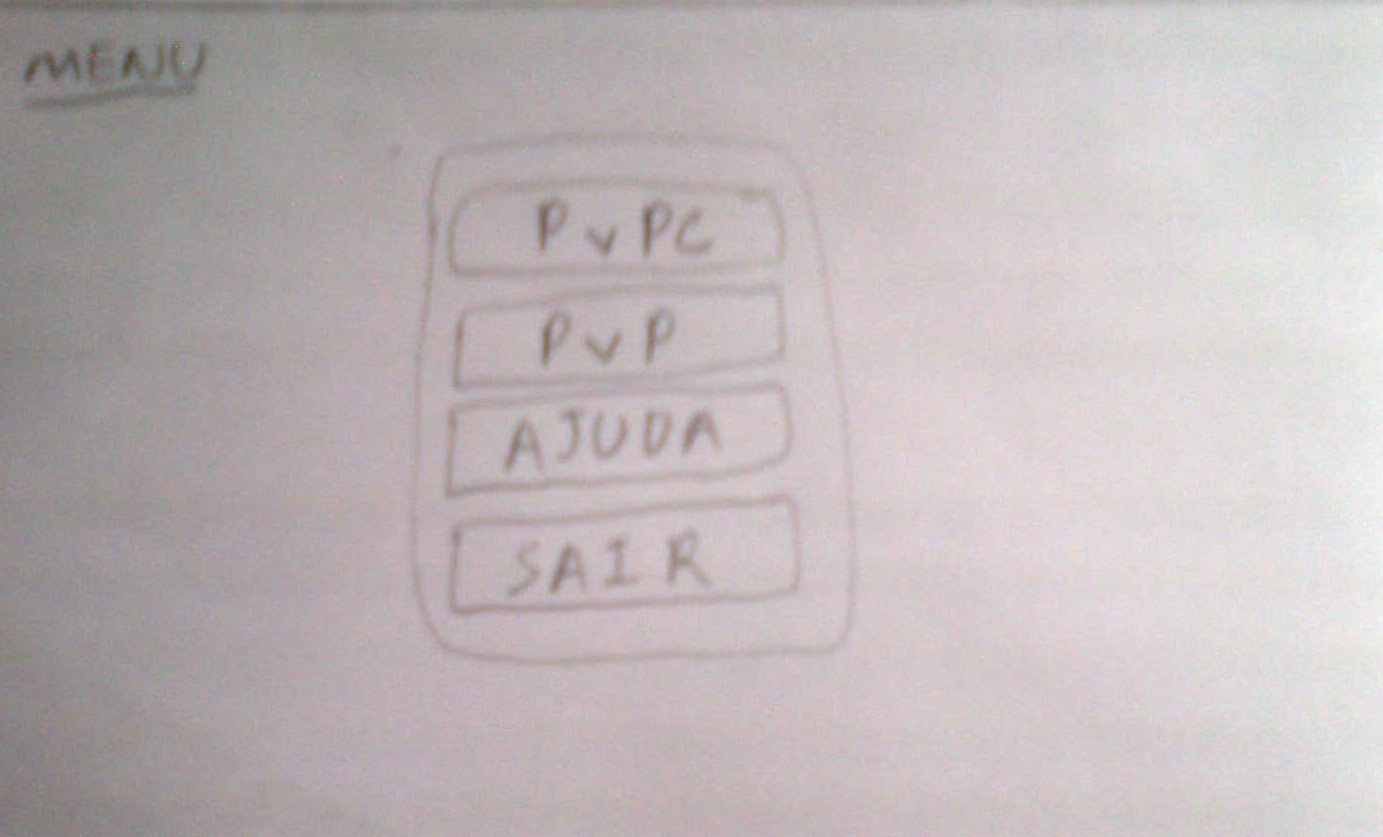
\includegraphics[width=0.7\textwidth]{menu}
\end{figure}

\subsection{Tabuleiro}
\label{subsec: tabuleiro}

\subsubsection{Sem realidade aumentada}
\label{subsubsec: semrealidadeaumentada}

\begin{figure}[h]
\centering
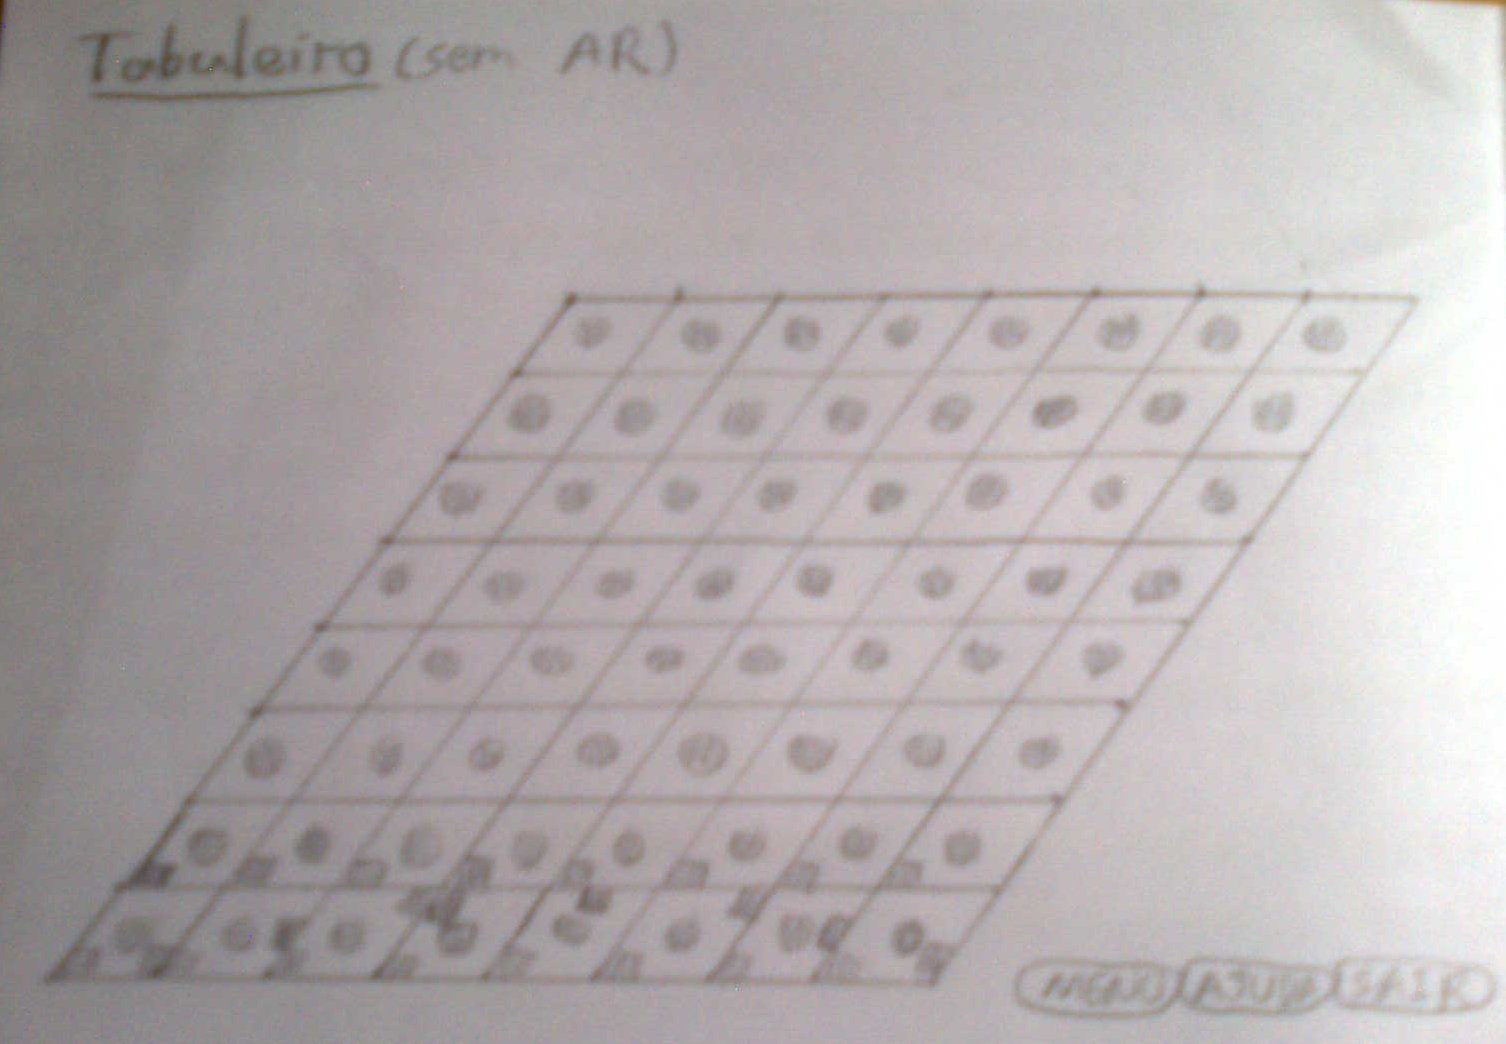
\includegraphics[width=0.7\textwidth]{tabuleirosemar}
\end{figure}

\subsubsection{Com realidade aumentada}
\label{subsubsec: comrealidadeaumentada}

\begin{figure}[h]
\centering
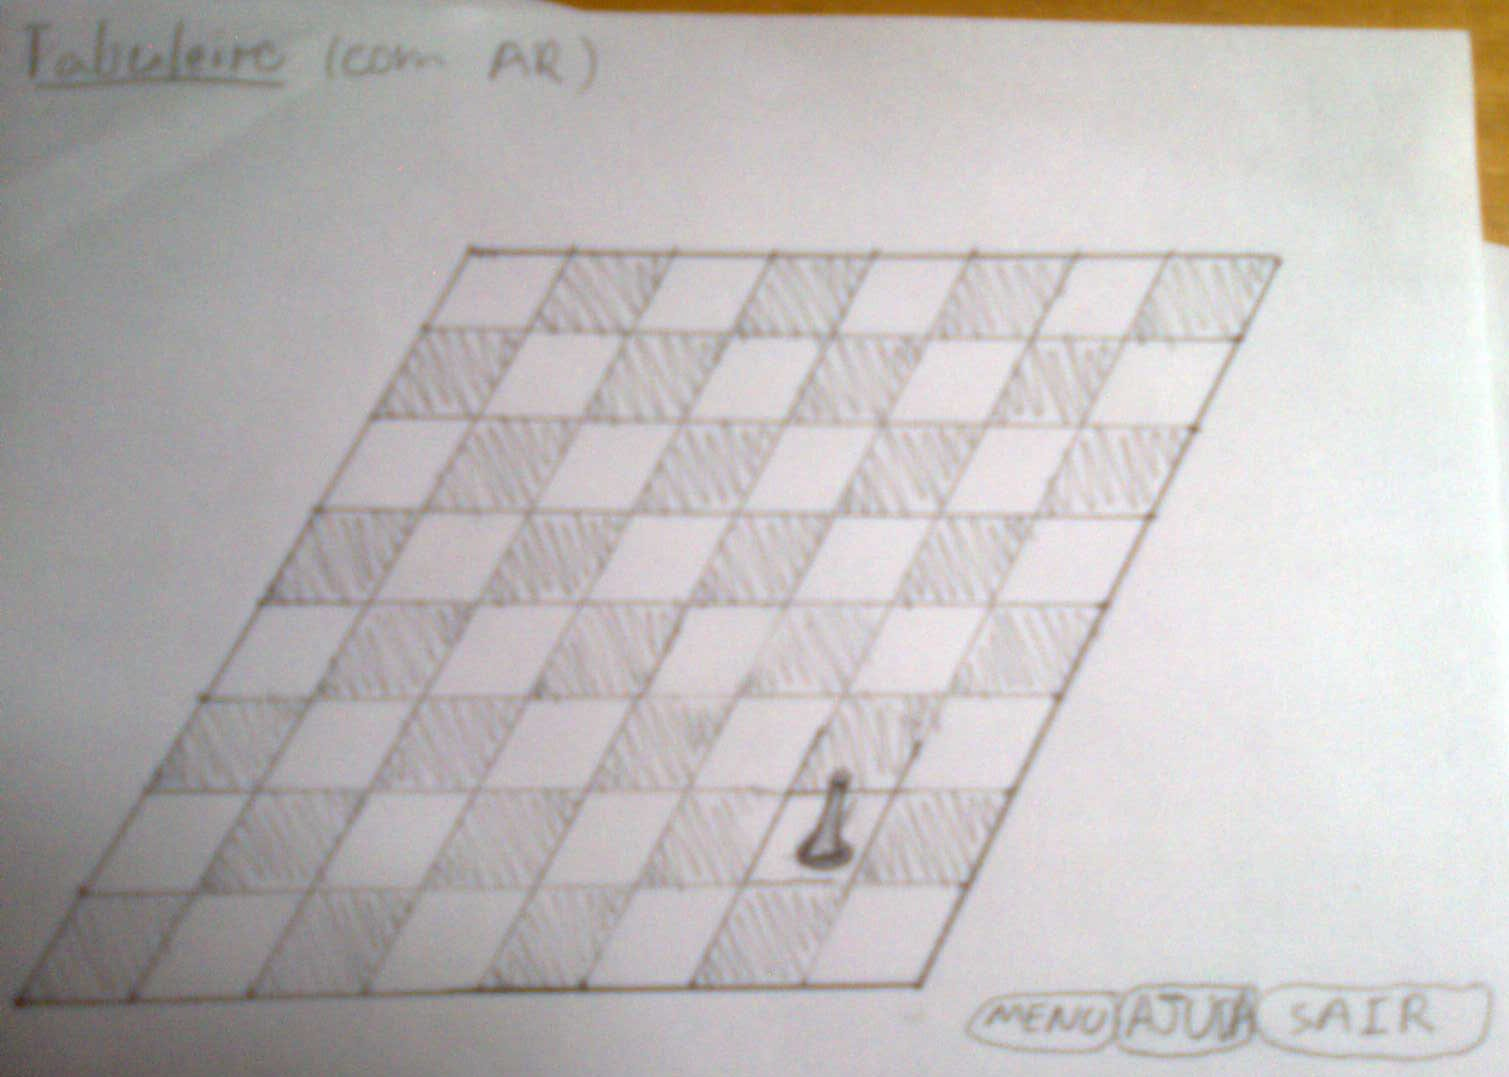
\includegraphics[width=0.7\textwidth]{tabuleirocomar}
\end{figure}

\subsection{Ajuda}
\label{subsubsec: ajuda}

\begin{figure}[h]
\centering
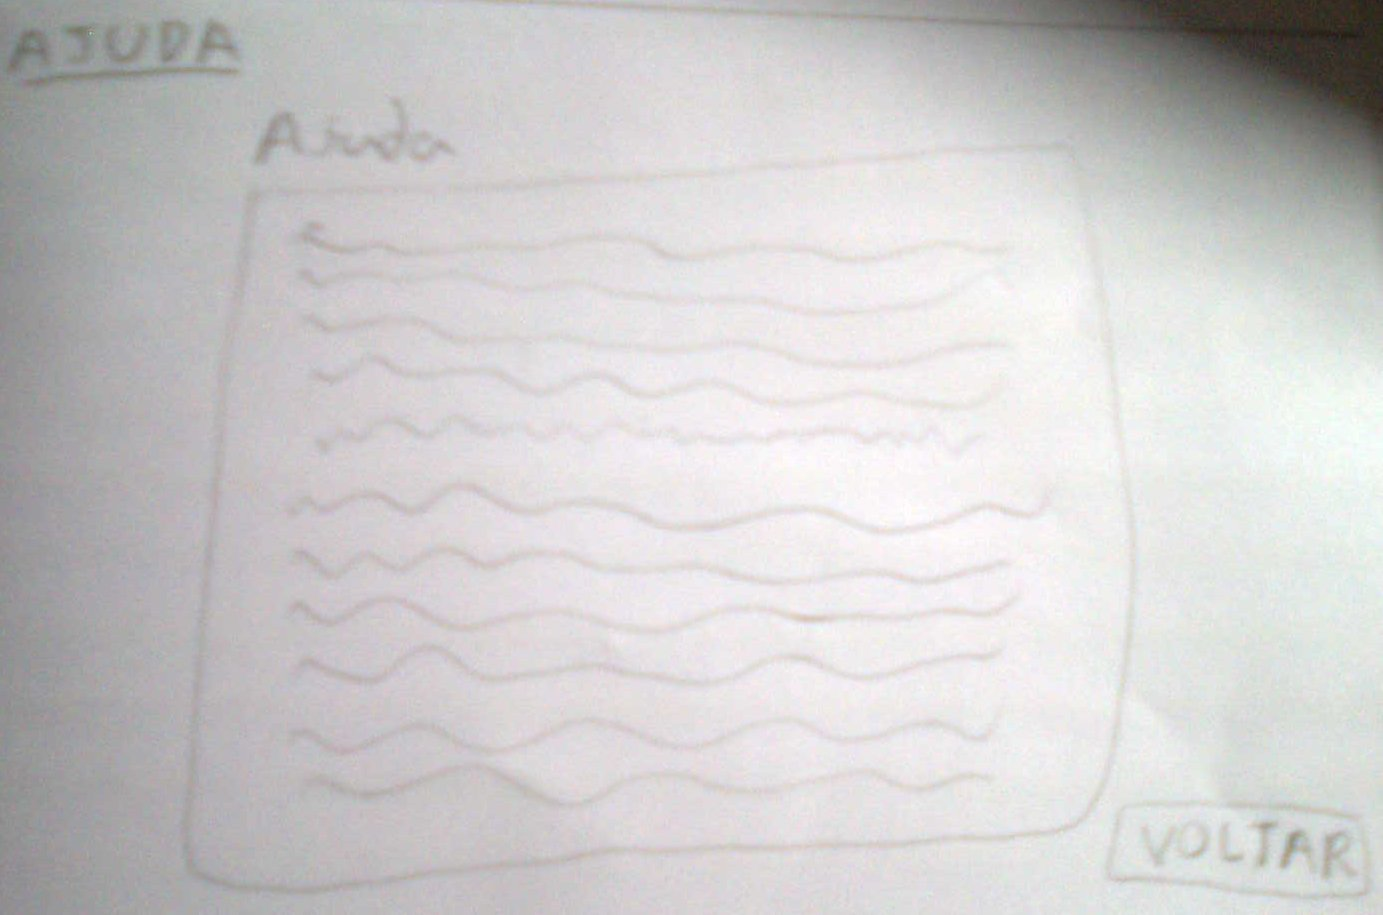
\includegraphics[width=0.7\textwidth]{ajuda}
\end{figure}

\newpage
\section{Considera\c c\~oes finais}
\label{sec: consideracoesfinais}

\subsection{Poss\'iveis dificuldades}
\label{subsec: possiveisdificuldades}

N\~ao esperamos que este projeto seja f\'acil devido a fatores como identificar
64 tags lado a lado que podem variar dentro de 9 tipos de tags e n\~ao devem ser
muito grandes (n\~ao mais que 3cm X 3cm) para preservar um m\'inimo de
jogabilidade.

\subsection{Funcionalidades b\^onus}
\label{subsec: funcionalidaesbinus}

A princ\'ipio, a \'unica funcionalidade extra que imaginamos \'e a anima\c c\~ao
da movimenta\c c\~ao das pe\c cas e a intera\c c\~ao entre elas que denpender\'a
do quanto tempo nos sobrar\'a e nossa habilidade com o Blender.

\subsection{Mais sobre o projeto}
\label{subsec; maissobreoprojeto}

Mais informa\c c\~oes sobre o projeto, como endere\c co do reposit\'orio de
c\'odigo e do gerenciador de tarefas, podem ser encontradas no blog do projeto:
\url{http://xadrezemrealidadeaumentada.blogspot.com/}.

Os esbo\c cos das telas (\ref{sec: telas}) tamb\'em podem ser encontrados em
alta resolu\c c\~ao no blog.

\end{document}